\documentclass[a4paper,12pt,oneside]{report}
\usepackage{titlesec}
\usepackage[svgnames]{xcolor}
%\usepackage[usenames,dvipsnames]{color}
\usepackage[top=0cm,bottom=0cm,left=0cm,right=0cm]{geometry}
%\usepackage{fullpage}
\usepackage[utf8]{inputenc}
\usepackage[T1]{fontenc}
\usepackage{graphicx}
\usepackage{wallpaper}
\usepackage{wrapfig}
\usepackage{hyperref}
\usepackage[francais]{babel}
%\usepackage{color}
\usepackage{layout}
\usepackage{circuitikz}
\usepackage[squaren, Gray]{SIunits}
\usepackage{sistyle}
\usepackage[autolanguage]{numprint}

%Algo package
\usepackage[ruled,vlined]{algorithm2e}
\usepackage{algpseudocode}

\usepackage{array}
\usepackage{calc}

\hypersetup{pdfborder={0 0 0}}

\titleformat{\part}
{\centering\fontfamily{pag}\fontsize{30}{30}\selectfont}
{\fontfamily{pag}\fontsize{30}{30}\selectfont Partie \ \thepart \ - }
{0pt}
{}{}

%Modifie le format des chapitres
\titleformat{\chapter}
{\it \color{DodgerBlue} \fontfamily{pag}\fontsize{20.74}{20}\selectfont}
{\it \fontfamily{pag}\fontsize{20.74}{20}\selectfont Chapitre \ \thechapter \ - }
{0pt}
{}{}
\titlespacing{\chapter}{0pt}{0.5cm}{0.5cm}[0pt]

%Modifie le format des sections
\titleformat{\section}
{\color{LimeGreen}\fontfamily{pag}\fontsize{15}{15}\selectfont}
{\fontfamily{pag}\fontsize{15}{15}\selectfont \thesection }
{5pt}
{}{}
\titlespacing{\section}{1cm}{0.5cm}{0.25cm}[0cm]

%Modifie le format des sous-secions
\titleformat{\subsection}
{\color{DarkOrange}\fontfamily{pag}\fontsize{12}{12}\selectfont}
{\fontfamily{pag}\fontsize{12}{12}\selectfont \thesubsection}
{5pt}
{}{}
\titlespacing*{\subsection}{2cm}{0.1cm}{0.1cm}[0cm]

%Modifie l'espace avant les paragraphes
\setlength{\parindent}{0pt}
\makeatletter

\newcommand{\bigO}{$\mathcal{O}$}

% Commande créeant une page de titre
%	#1=Titre
%	#2=Sous-titre
%	#3=Auteur
%	#4=image
%	#5=couleur de fond
%	#6=couleur cadre titre,sous-titre,auteur
\newcommand{\titre}[6]
{
	\begin{document}
	\begin{titlepage}
		\pagecolor{#5} % met la couleur de la page
		\vspace*{0.6cm}\fontfamily{pag}\fontsize{20}{20}\selectfont{\begin{center}2015-2016\end{center}}\vspace*{0.3cm}	% insère l'année en haut de la page
		\vspace*{-0.1cm}
		\includegraphics[width=\paperwidth]{#4} % insère l'image
		\colorbox{#6}{	%boîte de couleur avec le titre, sous-titre et l'auteur
			\hspace*{1.2cm}
			\begin{minipage}{\textwidth-1.8cm}{
				\vspace*{1cm}
				\begin{flushleft}\bfseries
					\fontfamily{pag}\fontsize{35}{35}\selectfont{#1}	%Titre
					\vspace*{0.5cm}
				\end{flushleft}
				\begin{flushleft}
					\fontfamily{pag}\fontsize{30}{30}\selectfont{#2}	%Sous-Titre
				\end{flushleft}
				\vspace*{1cm}
				\begin{flushright}
					\fontfamily{pag}\fontsize{20}{20}\selectfont{#3}	%Auteur
				\end{flushright}}
			\vspace*{1cm}
			\end{minipage}}
			\begin{center}
				\vfill % repli le reste de la page
				\fontfamily{pag}\fontsize{20}{20}\selectfont{\today} 	%Date
			\end{center}
	\end{titlepage} % fin de la page de titre
	\color{black} % met la couleur du reste du texte à noir
	\pagecolor{white}	% met la couleur des pages suivante à blanc
	\newgeometry{top=1.5cm,bottom=1.5cm,left=1cm,right=1cm}	% modification des marges
	\tableofcontents	%tables des matières
}
 \titre{ELEC - 1350\\Électromagnétisme}{Synthèse}{Damien Deprez}{PageDeGardeF}{LightBlue}{LightGreen}
 \chapter{Force et champ électrostatique}
 \section{Loi de Coulomb}
 \textbf{Force entre deux charges} $$\vec{F} = \frac{Q_1Q_2}{4\pi\epsilon_0R_{12}^2} \vec{a}_{12}$$
 avec
 \begin{itemize}
  \item $R_{12} \unit{}{\left[\meter \right]}$ la distance entre les deux charges
  \item $\epsilon_0 = 1/36\pi 10^{-9} \unit{}{\left[ \farad/\meter\right]}$
  \item $\vec{a}_{12}$ vecteur direction de $1$ à $2$.
 \end{itemize}
 \textbf{Champ} $$\vec{E} = \frac{\vec{F}_t}{Q_t}$$
 
 \textbf{Sens du champ électrique}
 \begin{center}
  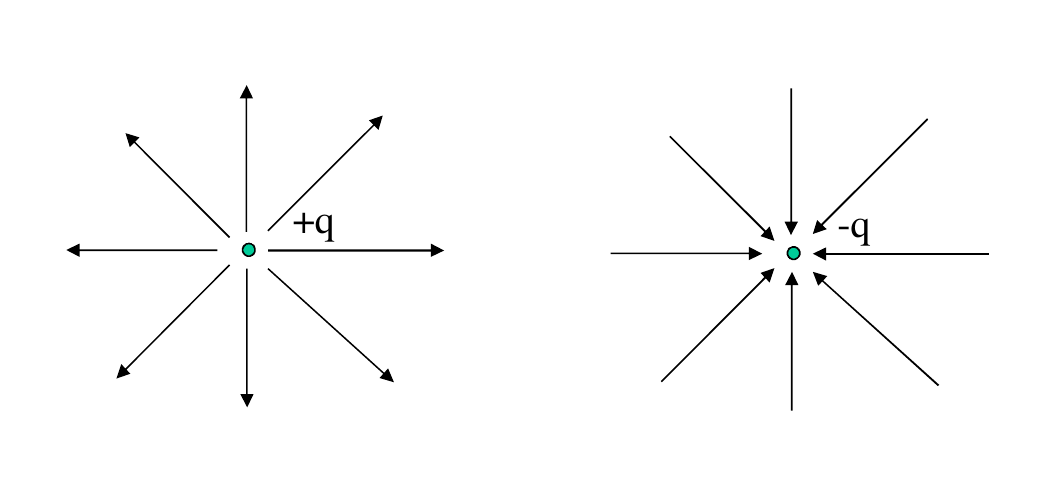
\includegraphics[width=0.7\textwidth]{SensChampE}
 \end{center}
 Le champ électrique est \emph{vectoriel} et \emph{radial} par rapport à la charge ponctuelle qui le crée. Le principe de superposition s'applique au champ électrique.\\
 \textbf{Type de charge}
 \begin{itemize}
  \item charge ponctuelle
  \item charge linéique $\rho_l$
  \item charge surfacique $\rho_s$
  \item charge volumique $\rho_v$
 \end{itemize}
 \textbf{Champ dû à une distribution de charge dans le vide}
 $$\vec{E}(r)= \int_{vol}{\frac{\rho_v(\vec{r'})dv}{4\pi\epsilon_0 |\vec{r} - \vec{r'}|^2}\frac{\vec{r}-\vec{r'}}{|\vec{r}-\vec{r'}|}}$$
 où $\rho_v(\vec{r'})dv$ est la charge contenue dans le volume.\\
 \textbf{Champ de déplacement d'une charge ponctuelle}
 $$\vec{D} = \frac{Q}{4\pi r^2}\vec{a}_{r} = \epsilon_0 \vec{E}$$
\end{document}
